%%% Local Variables: 
%%% mode: latex
%%% TeX-master: prova
%%% End: 

\question{2 pontos}
Calcular o tempo médio de escrita e leitura de um setor para um disco
rígido com as características relacionadas na Tabela~\ref{tab:disk}:

\begin{table}[ht]
\begin{center}
\begin{tabular}{|c|p{2.2cm}|c|p{2.2cm}|p{2.2cm}|p{2.2cm}|}\hline
  & \footnotesize Tempo médio de busca &  Rotação &  \footnotesize
  Taxa de transferência do disco  & \footnotesize Taxa de
  transferência da controladora  & \footnotesize Tamanho do setor\\\hline
  \bf a. & 8 ms & 7200 RPM & 32MBytes/s & 320 Mbits/s & 1024 bytes\\\hline
\end{tabular}
\caption{Características de 1 sistema com disco rígido.}
\label{tab:disk}
\end{center}
\end{table}

\noindent O tempo de atraso da controladora é calculado utilizando a
taxa de transferência da controladora.

\question{2 pontos} Calcular o tempo médio para
ler um setor de 1024 bytes na memória listada na
Tabela~\ref{tab:flash}.

\begin{table}[ht]
  \centering
  \begin{tabular}[ht]{|c|c|c|}\hline
    & \footnotesize Taxa de transferência de dados&
    \footnotesize Taxa de transferência do controlador\\\hline
    \bf a. & 34 MB/s & 480 MB/s\\\hline
  \end{tabular}
  \caption{Características de duas memórias flash.}
  \label{tab:flash}
\end{table}


\question{4}
A listagem a seguir contem uma lista de referências para endereços
de memória DRAM de {\bf 4} bits.

\begin{center}
  \tt
 \rand\arabic{rand} \rand\arabic{rand}
 \rand\arabic{rand} \rand\arabic{rand} \rand\arabic{rand} \rand\arabic{rand}
 \rand\arabic{rand} \rand\arabic{rand}
 %\rand\arabic{rand} \rand\arabic{rand} \\
\end{center}

Para cada uma das referências, realizar os seguintes mapeamentos para
a memória cache (SRAM) com quatro endereços (índices {\tt 00, 01, 10, 11}):

\begin{itemize}
\item{\tiny [1 ponto]} Mapeamento associativo {\bf direto};
\item{\tiny [1 ponto]} {\bf Mapeamento associativo em conjunto com duas vias}, utilizando o
  algoritmo {\bf LRU} (Último usado recentemente) para
  reposição dos blocos na memória cache (SRAM);
\item{\tiny [1 ponto]} {\bf Sem mapeamento}, utilizando o algoritmo {\bf LRU} para
  reposição dos blocos na memória cache (SRAM);
\end{itemize}

\noindent{\tiny [1 ponto]} Calcular a taxa de {\em miss} e {\em hit}
durante a requisição dos endereços de memória DRAM.

\question{1} O que é interrupção de Entrada/Saída (E/S) na comunicação
entre os dispositivos de E/S e o processador?

\question{1} Como é e quais são as vantagens dos dispositivos de E/S que têm suporte a
acesso direto à memória (DMA--\emph{Direct Memory Access})?


\paragraph{Questão \newex{}. (10 pontos)}
A listagem a seguir contem uma lista de referências para endereços
de memória DRAM de {\bf 5} bits.

\begin{center}
  \tt
 \rand\arabic{rand} \rand\arabic{rand}
 \rand\arabic{rand} \rand\arabic{rand} \rand\arabic{rand} \rand\arabic{rand}
 \rand\arabic{rand} \rand\arabic{rand} \rand\arabic{rand} \rand\arabic{rand} \\
\end{center}

Para cada uma das referências, realizar os seguintes mapeamentos para
a memória cache (SRAM), conforme ilustrado na Figura~\ref{fig:mmap}:

\begin{itemize}
\item{\tiny [2 pontos]} Mapeamento associativo {\bf direto};
\item{\tiny [2 pontos]} {\bf Mapeamento associativo em conjunto com duas vias}, utilizando o
  algoritmo {\bf LRU} (Último usado recentemente) para
  reposição dos blocos na memória cache (SRAM);
\item{\tiny [2 pontos]} {\bf Mapeamento associativo em conjunto com duas
  vias}, utilizando o algoritmo {\bf aleatório }
  para reposição dos blocos na memória cache (SRAM);
\item{\tiny [2 pontos]} {\bf Sem mapeamento}, utilizando o algoritmo {\bf LRU} para
  reposição dos blocos na memória cache (SRAM);
\item{\tiny [2 pontos]} {\bf Sem mapeamento}, utilizando o algoritmo {\bf aleatório } para
  reposição dos blocos na memória cache (SRAM);
\end{itemize}


\newcounter{dramaddr}\setcounter{dramaddr}{0}

\begin{figure}
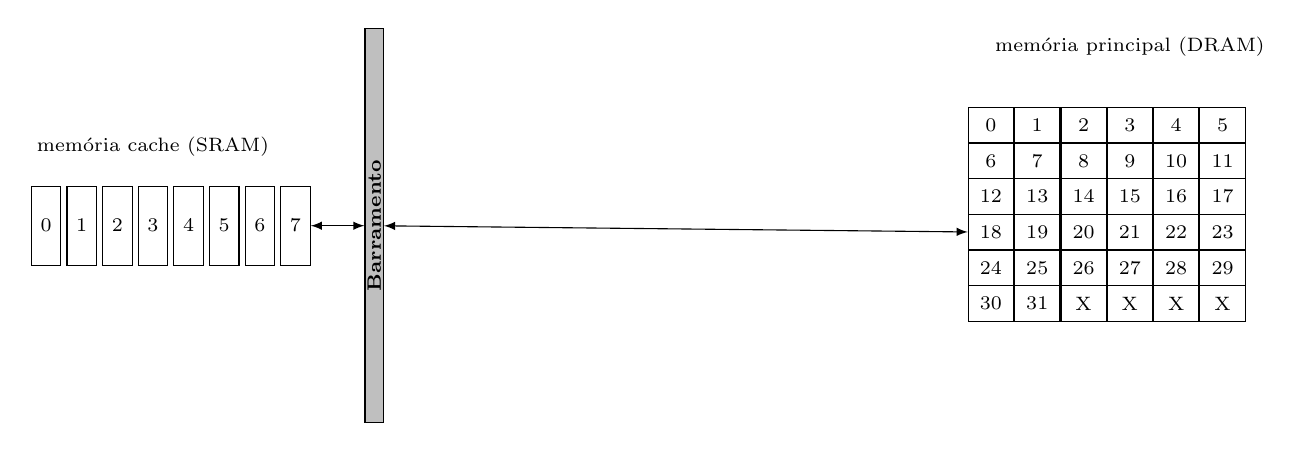
\begin{tikzpicture}[font=\scriptsize]
  \foreach \x in {0,...,7} {
    \node[minimum height=1cm, draw] (c\x) at (\x/2.21,0) [below] {\scriptsize \x};
  }
  \node [minimum height=5cm, right of=c7, fill=lightgray, draw] (bus)
  {};
  \node[rotate=90] at (bus) {\bf Barramento};
  \node [above of=c3] {memória cache (SRAM)};

%  \foreach \x in {1,3,5,7} {
 %   \draw (c\x)+(0.0,0cm) -- (c\x)+(0.0cm,4cm);
 % }

  \foreach \y in {0,...,5} {
    \foreach \x in {0,...,5} {
      \def\addr{\arabic{dramaddr}}
     
      \node[minimum height=.45cm, minimum width=.575cm, draw] (m\x\y) at
      (12+\x/1.7,1-\y/2.21) [below] {\scriptsize \ifnum\addr<32 \addr
      \else X \fi};
      \addtocounter{dramaddr}{1}
    }
  }

    \path[<->,>=latex,draw] (c7) -- (bus);
    \path[<->,>=latex,draw] (bus) -- (m03);
\node [above of=m30] {memória principal (DRAM)};
\end{tikzpicture}
\caption{Comunicação entre memória cache (SRAM) de 4 blocos, com 2 palavras
  cada, e memória principal (DRAM) com 32 endereços.}
\label{fig:mmap}
\end{figure}


A Tabela~\ref{tab:refs} contem uma lista de referências para endereços
de memória de 6 bits.

\begin{table}[h]
\centering
\begin{tabular}{|l|l|}\hline
  \bf a. & 0, 34, 12, 0, 35, 13, 62, 61, 2, 44, 0, 21 \\\hline
\end{tabular}
\caption{Tabela de referências para duas requisições de endereços para
  a memória cache.}
\label{tab:refs}
\end{table}

Para cada uma das referências da Tabela~\ref{tab:refs}, realizar os
{\bf mapeamentos direto e associativo em duas vias} de uma cache com {\bf 8}
blocos. Também listar se cada referência requisitada apresenta {\it
  cache hit/miss\/} calculando a taxa de ausência de endereços. Assumir
que inicialmente a cache está vazia.

\pagebreak

\vfill
\paragraph{Questão \newex{}. (0,5 ponto)}
Qual das afirmações abaixo não é aplicável à memória de acesso aleatório
estática (SRAM) quando comparada com a memória de acesso aleatório
dinâmica (DRAM):
{\footnotesize
\pgfkeyssetvalue{/sramxdram/0}{\item Alto custo.}
\pgfkeyssetvalue{/sramxdram/1}{\item Grande capacidade de armazenamento.}
\pgfkeyssetvalue{/sramxdram/2}{\item Alto consumo de energia.}
\pgfkeyssetvalue{/sramxdram/3}{\item Não há necessidade de pulsos de {\em refresh}.}
\pgfkeyssetvalue{/sramxdram/4}{\item Tempo de acesso pequeno.}

\begin{enumerate}[(a)]%
\foreach \i in \thelist
{\pgfkeysvalueof{/sramxdram/\i}}
\end{enumerate}
}

\paragraph{Questão \newex{}. (0,5 ponto)}
Qual das afirmações abaixo não é aplicável à memória de acesso aleatório
dinâmica (DRAM) quando comparada com a memória de acesso aleatório
estática (SRAM):

{\footnotesize
\pgfkeyssetvalue{/dramxsram/0}{\item Baixo custo.}
\pgfkeyssetvalue{/dramxsram/1}{\item Grande capacidade de armazenamento.}
\pgfkeyssetvalue{/dramxsram/2}{\item Baixo consumo de energia.}
\pgfkeyssetvalue{/dramxsram/3}{\item Não há necessidade de pulsos de {\em refresh}.}
\pgfkeyssetvalue{/dramxsram/4}{\item São usados capacitores para sua construção.}

\begin{enumerate}[(a)]%
  \foreach \i in \thelist
  {\pgfkeysvalueof{/dramxsram/\i}}
\end{enumerate}
}

\paragraph{Questão \newex. (0,5 ponto)} A tabela de páginas
localiza-se no (a):

\pgfkeyssetvalue{/page/0}{\item Memória cache.}
\pgfkeyssetvalue{/page/1}{\item Registrador.}
\pgfkeyssetvalue{/page/2}{\item Disco R$\acute{i}$gido.}
\pgfkeyssetvalue{/page/3}{\item Memória principal (DRAM).}
\pgfkeyssetvalue{/page/4}{\item Memória ROM.}

\begin{enumerate}[(a)]
  \foreach \i in \thelist
  {\pgfkeysvalueof{/page/\i}}
\end{enumerate}


\paragraph{Questão \newex. (0,5 ponto)} A tabela de páginas armazena
informações a respeito do mapeamento entre os endereços lógicos e
físicos de memória. Há um campo de tamanho de 1 bit nesta tabela que
informa se a página está na memória física ou disco rígido. Este bit é
chamado de:

\pgfkeyssetvalue{/bit/0}{\item referência}
\pgfkeyssetvalue{/bit/1}{\item sujeira}
\pgfkeyssetvalue{/bit/2}{\item bloqueio}
\pgfkeyssetvalue{/bit/3}{\item validade}
\pgfkeyssetvalue{/bit/4}{\item paginação}

\begin{enumerate}[(a)]
  \foreach \i in \thelist
  {\pgfkeysvalueof{/bit/\i}}
\end{enumerate}


\paragraph{Questão \newex. (0,5 ponto)} Associe cada número de RAID
({\em Redundant Array of Inexpensive Disks})
dos itens a seguir com a sua descrição no lado direito.
\bigskip

\pgfkeyssetvalue{/raid/0}{  \item[RAID $\underline{\hbox{\ \ \ }}$]: Entrou em desuso.}
\pgfkeyssetvalue{/raid/1}{  \item[RAID $\underline{\hbox{\ \ \ }}$]: Há redundância de cada
    disco. Se um disco falhar, o disco redundante entra em ação.}
\pgfkeyssetvalue{/raid/2}{  \item[RAID $\underline{\hbox{\ \ \ }}$]: Não há necessidade de ter
    um disco redundante para cada disco do RAID, pois um ou mais
    discos atuam armazenando informações de paridade de bit dos
    discos. Em caso de falha, é feita a reconstrução do dado do disco
    com problemas a partir dos bits de paridade dos discos.}
\pgfkeyssetvalue{/raid/3}{  \item[RAID $\underline{\hbox{\ \ \ }}$]: Não há redundância, os
    discos apenas são agrupados fornecendo ao sistema operacional a
    visão de um único disco.}
\pgfkeyssetvalue{/raid/4}{  \item[RAID $\underline{\hbox{\ \ \ }}$]: Não há necessidade de ter
    um disco redundante para cada disco do RAID, pois um ou mais
    discos atuam armazenando informações de paridade de bloco de cada
    disco. Em caso de falha, é feita a reconstrução do dado do disco
    com problemas a partir dos blocos de paridade do disco que falhou.}

\begin{description}
  \foreach \i in \thelist
  {\pgfkeysvalueof{/raid/\i}}
\end{description}
  
\paragraph{Questão \newex{}. (0,5 ponto)}
A memória de acesso somente-leitura (ROM) não é volátil contendo um
padrão permanente de dados que não pode ser mudado. Qual das
aplicações a seguir normalmente não é armazenada na memória ROM?

\pgfkeyssetvalue{/rom/0}{\item Programas do sistema.}
\pgfkeyssetvalue{/rom/1}{\item Micro-programação.}
\pgfkeyssetvalue{/rom/2}{\item Tabelas de funções.}
\pgfkeyssetvalue{/rom/3}{\item Biblioteca de funções de uso frequente.}
\pgfkeyssetvalue{/rom/4}{\item Sistema operacional.}

\begin{enumerate}[(a)]
  \foreach \i in \thelist
  {\pgfkeysvalueof{/rom/\i}}
\end{enumerate}

\paragraph{Questão \newex{}. (0,5 ponto)}
Qual das características a seguir não é aplicável à memória
programável ROM apagável (EPROM):

\pgfkeyssetvalue{/eprom/0}{\item São utilizados capacitores para sua construção.}
\pgfkeyssetvalue{/eprom/1}{\item Os dados são lidos e gravados eletricamente.}
\pgfkeyssetvalue{/eprom/2}{\item Antes da operação de escrita todas as células precisam ser apagadas;}
\pgfkeyssetvalue{/eprom/3}{\item A operação de apagamento é feita utilizando luz ultravioleta;}
\pgfkeyssetvalue{/eprom/4}{\item Não necessita de pulsos de {\em refresh}.}

\begin{enumerate}[(a)]
  \foreach \i in \thelist
  {\pgfkeysvalueof{/eprom/\i}}
\end{enumerate}

\paragraph{Questão \newex{}. (0,5 ponto)}
Qual das características a seguir não é aplicável à memória
programável ROM apagável eletricamente (EEPROM):

\pgfkeyssetvalue{/eeprom/0}{\item Utilizada principalmente para leitura.}
\pgfkeyssetvalue{/eeprom/1}{\item Mais densa que a memória EPROM.}
\pgfkeyssetvalue{/eeprom/2}{\item A gravação é feita sem apagamento de todo o conteúdo.}
\pgfkeyssetvalue{/eeprom/3}{\item Na gravação somente o byte ou bytes endereçados são atualizados.}
\pgfkeyssetvalue{/eeprom/4}{\item Mais cara que a EPROM.}

\begin{enumerate}[(a)]
  \foreach \i in \thelist
  {\pgfkeysvalueof{/eeprom/\i}}
\end{enumerate}

\paragraph{Questão \newex{}. (0,5 ponto)}
Qual das características a seguir não é aplicável à memória
{\em flash}:

\pgfkeyssetvalue{/flash/0}{\item Intermediária entre a EPROM e EEPROM.}
\pgfkeyssetvalue{/flash/1}{\item Utiliza tecnologia elétrica de apagamento.}
\pgfkeyssetvalue{/flash/2}{\item Oferece apagamento em n$\acute{i}$vel de byte.}
\pgfkeyssetvalue{/flash/3}{\item É possivel apagar blocos de memória ao invés da memória inteira.}
\pgfkeyssetvalue{/flash/4}{\item O {\em pendrive} é um exemplo de dispositivo que a utiliza.}


\begin{enumerate}
  \foreach \i in \thelist
  {\pgfkeysvalueof{/flash/\i}}
\end{enumerate}
